\chapter{Arquitetura do \textit{framework} de simulação}

Uma vez definida a arquitetura de \textit{middleware} de comunicação a ser utilizado durante este projeto, o próximo passo é a definição do funcionamento e da arquitetura da camada de simulação, aqui genericamente denominado \textit{framework}.

Esta camada, conforme ilustrada na figura~\ref{fig:camada_central}, compreende diversos sub-componentes do framework (aqui esses sub-componentes serão denominados genericamentes de blocos, para que se distingua dos componentes, objetos utilizados para descrever um modelo a ser simulado). Cada bloco que compreende o kernel se liga ao bloco central, denominado \textit{kernel}. Este é o responsável por coordenar a simulação, aplicando sincronização e balanceamento de carga, além de gerenciar o ciclo de vida da simulação (quando começar, quando terminar, etc).

\begin{figure}
  \centerline{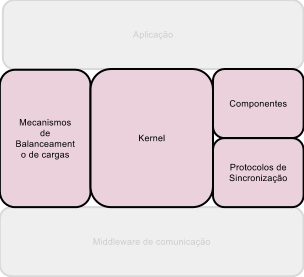
\includegraphics{camada_framework.png}}
  \caption{A camada aqui denominada \textit{framework}.}
\label{fig:camada_central}
\end{figure}

\section{O bloco Componente}

Um componente é uma abstração de um comportamento que desejamos reproduzir na nossa simulação. Na abstração de um sistema de caixa de supermercados, por exemplos, pode-se extrair três componentes (que são comuns em muitas situações na simulação de eventos discretos): o produtor, a fila de espera e o consumidor.

Uma biblioteca de componentes deve proporcionar objetos parametrizáveis que permitam a descrição do comportamento de cada um deles. No caso citado anteriormente, o componete produtor deve suportar parâmetros que, por exemplo, descreva a taxa de criação de novos evento, e as características de cada evento criado.

O componente é construido diretamente em cima do objeto \textit{process}, construído na camada de comunicação. Isso garante ao componente criado, por herança direta, toda funcionalidade de comunicação entre outros componentes. Desta maneira, basta ao usuário do framework descrever na modelagem qual a conexão que cada componente faz, que esta é reproduzida automaticamente pelo framework, independente se esses componentes são processo cohabitantes ou não-cohabitantes.

\section{O \textit{kernel} do \textit{framework}}
\section{Protocolos de sincronização}
\section{Algoritmos de balanceamento de carga}
